%
%   ADICIONAR REFERÊNCIAS NESTE CAPÍTULO
%
\chapter{Gestão e planejamento}\label{cap:gestao}

O total de horas estimadas para desenvolvimento do projeto foi calculada através do método de \textit{Use Case Points}, que baseia-se em informações extraídas diretamente dos diagramas de Casos de Uso especificados.

O presente capítulo mostra todos os passos desenvolvimentos para o cálculo dos \textit{Use Case Points}, bem como a utilização dos métodos \sigla{PERT}{\textit{Program Evaluation and Review Technique}} (\textit{Program Evaluation and Review Technique}) e \sigla{CPM}{\textit{Critical Path Method}} (\textit{Critical Path Method}) para elaboração da Rede PERT-CPM, pela qual é possível observar o caminho crítico para o desenvolvimento do projeto, usando como base as tarefas e suas horas estipuladas.

\section{\textit{Use Case Points}}

A estimativa por \textit{Use Case Points} consiste em alguns passos. \citeonline{clemmons} exemplificou os passos para o cálculo do \textit{Use Case Points}, os quais serão seguidos neste capítulo.

O primeiro passo é calcular o \sigla{UAW}{\textit{Unadjusted Actor Weight}} (\textit{Unadjusted Actor Weight}), o peso total dos atores do sistema. Os atores foram classificados como: ator complexo (Usuário), com peso 3 e ator médio (Aplicativo móvel), com peso 2.

\begin{center}
UAW = 3x1 + 2x1 = 5
\end{center}

Em seguida, calcula-se o peso não-ajustado de cada Caso de Uso do sistema. Os casos de uso foram classificados da seguinte forma:

\begin{itemize}
\item Coletar coordenada: caso de uso médio (peso 10).
\item Armazenar informações: caso de uso médio (peso 10).
\item Enviar informações: caso de uso complexo (peso 15).
\item Receber informações: caso de uso médio (peso 10).
\item Procurar por dispositivos: caso de uso médio (peso 10).
\end{itemize}

O \sigla{UUCW}{\textit{Unadjusted Use Case Weight}} (\textit{Unadjusted Use Case Weight}) é então calculado:

\begin{center}
UUCW = 10x3 + 15x2 = 60
\end{center}

No terceiro passo, calcula-se o \sigla{UUCP}{\textit{Unadjusted Use Case Point}} (\textit{Unadjusted Use Case Point}), que consiste na soma de UAW com UUCW:

\begin{center}
UUCP = UAW + UUCW = 65
\end{center}

Prossegue-se então para o cálculo de fatores técnicos, que cobre requisitos funcionais do sistema, e fatores de ambiente, que cobre requisitos não-funcionais associados ao processo de desenvolvimento.

A variável de fatores técnicos, TFactor, é obtida através do somatório dos níves F1 a F13, multiplicados pelo seu peso:

\begin{table}[h!]
\caption[Fatores técnicos]{Fatores técnicos. Fonte: Autoria própria.}
\begin{center}
%\scalebox{0.75}{
\begin{tabular}{|c|c|c|c|c|}
\hline
\textbf{Fator} & \textbf{Fatores que contribuem para a complexidade} & \textbf{Peso} & \textbf{Valor}  & \textbf{Total} \\ \hline \hline
F1  & Sistemas distribuídos & 2 & 5 & 10	\\
\hline
F2  & Tempo de resposta & 1 & 5 & 5	\\
\hline
F3  & Eficiência para o usuário final (on-line) & 1 & 5 & 5	\\
\hline
F4  & Processamento interno complexo & 1 & 4 & 4	\\
\hline
F5  & Código reusável & 1 & 2 & 2	\\
\hline
F6  & Facilidade de instalação & 0,5 & 1 & 0,5	\\
\hline
F7  & Facilidade de uso (facilidade operacional) & 0,5 & 4 & 2	\\
\hline
F8  & Portabilidade & 2 & 3 & 6	\\
\hline
F9  & Facilidade de mudança & 1 & 3 & 3	\\
\hline
F10  & Concorrência (acesso simultâneo à aplicação) & 1 & 4 & 4	\\
\hline
F11  & Recursos de segurança & 1 & 3 & 3	\\
\hline
F12  & Fornece acesso direto para terceiros & 1 & 0 & 0	\\
\hline
F13  & Requer treinamento especial para o usuário & 1 & 0 & 0	\\
\hline
TFactor & & & & 44,5	\\
\hline
\end{tabular}%}
\end{center}
\label{tab:tfactor}
\end{table}

O \sigla{TCF}{\textit{Technical Complexity Factor}} (\textit{Technical Complexity Factor}) é então calculado:

\begin{center}
TCF = 0,6 + (0,01 x TFactor) = 0,6 + (0,01 x 44,5) = 1,045
\end{center}

\newpage

A variável de fatores de ambiente, EFactor, é calculada através do somatório dos níveis F1 a F8, multiplicados pelo seu peso:

\begin{table}[h!]
\caption[Fatores de ambiente]{Fatores de ambiente. Fonte: Autoria própria.}
\begin{center}
%\scalebox{0.75}{
\begin{tabular}{|c|m{9cm}|c|c|c|}
\hline
\textbf{Fator} & \textbf{Fatores que contribuem para a complexidade} & \textbf{Peso} & \textbf{Valor}  & \textbf{Total} \\ \hline \hline
F1  & Familiaridade da equipe com o processo formal de desenvolvimento adotado & 1,5 & 4 & 6	\\
\hline
F2  & Colaboradores de meio período & -1 & 2 & -2	\\
\hline
F3  & Capacidade do líder de projeto em análise de requisitos e modelagem & 0,5 & 4 & 2	\\
\hline
F4  & Experiência da equipe em desenvolvimento de aplicações do gênero em questão & 0,5 & 5 & 2,5	\\
\hline
F5  & Experiência em orientação a objetos & 1 & 5 & 5	\\
\hline
F6  & Motivação da equipe & 1 & 5 & 5	\\
\hline
F7  & Dificuldades com a linguagem de programação & -1 & 3 & -3	\\
\hline
F8  & Requisitos estáveis & 2 & 3 & 6	\\
\hline
EFactor & & & & 21,5	\\
\hline
\end{tabular}%}
\end{center}
\label{tab:efactor}
\end{table}

O \sigla{EF}{\textit{Environmental Factor}} (\textit{Environmental Factor}) é então calculado:

\begin{center}
EF = 1,4 + (-0,03 x EFactor) = 1,4 + (-0,03 x 21,5) = 0,755
\end{center}

Com os resultados obtidos nos passos anteriores, O valor de \sigla{UCP}{\textit{Use Case Points}} (\textit{Use Case Points}) pode ser então calculado:

\begin{center}
UCP = UUCP x TCF x EF = 51,28
\end{center}

O tempo de trabalho estimado pode ser obtido multiplicando-se UCP por 20. Portanto, estimou-se 1025,6 horas de trabalho.

\newpage

\section{Gerenciamento de tempo}

Para a elaboração da Rede PERT-CPM foi necessário, primeiramente,
levantar as tarefas do projeto em questão. As tarefas levantadas, bem como a duração de cada uma delas podem ser observadas na Tabela  \ref{tab:tarefas}:

\begin{table}[h!]
\caption[Tarefas do projeto]{Tarefas do projeto. Fonte: Autoria própria.}
\begin{center}
%\scalebox{0.75}{
\begin{tabular}{|c|m{10cm}|c|}\hline
\Centering\bfseries \textbf{Número} & \Centering\bfseries \textbf{Tarefa} & \Centering\bfseries \textbf{Duração}
%\textbf{Número} & \textbf{Tarefa} & \textbf{Duração} 
\\ \hline \hline
1 & Estudo de APIs e do Android SDK & 100	\\
\hline
2 & Projeto de software (modelagem UML) & 100	\\
\hline
3 & Implementação do projeto de software & 280	\\
\hline
4 & Testes do protótipo utilizando um dispositivo móvel
(emulado) com sistema operacional Android & 60	\\
\hline
5 & Testes do protótipo utilizando um dispositivo móvel (real)
com sistema operacional Android & 100	\\
\hline
6 & Finalização do artefato  & 192	\\
\hline
7 & Testes e ajustes finais no software  & 104	\\
\hline
8 & Finalização da documentação & 80	\\
\hline
9 & Preparação da apresentação para banca  & 8	\\
\hline
Total & & 1024	\\
\hline
\end{tabular}%}
\end{center}
\label{tab:tarefas}
\end{table}

Utilizando-se dos resultados expostos, a Rede PERT-CPM para o projeto é mostrada na Figura \ref{fig:pertcpm}.

\begin{figure}[h]
\begin{center}
    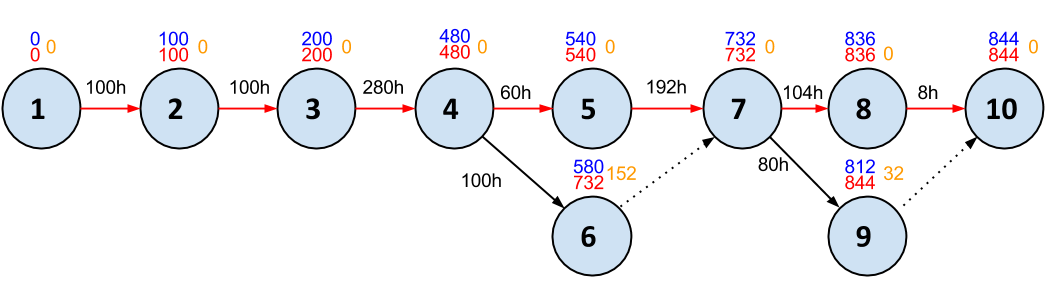
\includegraphics[width=1\columnwidth]{../figs/pert-cpm.png}
    \caption{Rede PERT-CPM.}Fonte: Autoria própria.%\cite{sujatha}
    \label{fig:pertcpm}
\end{center}
\end{figure}

Na figura, o ``cedo" de cada evento é evidenciado na cor azul, ao passo que o ``tarde" de cada evento é evidenciado na cor vermelha. A folga, diferença entre tarde e cedo, é apresentada na cor laranja/amarelo.

O caminho crítico fica destacado pelas setas em vermelho, e perpassa pelos eventos 1, 2, 3, 4, 5, 7, 8 e 10 e, por consequência, pelas tarefas 1, 2, 3, 4, 6, 7 e 9.